\documentclass[../main/main.tex]{subfiles}
\graphicspath{{./figures/}}

\makeatletter
\renewcommand{\@chapapp}{Travaux pratiques -- TP}
\makeatother

\toggletrue{student}
\HideSolutionstrue

\begin{document}
\setcounter{chapter}{3}

\chapter{Goniom\`etre \`a r\'eseau~: spectrom\'etrie}

\ifstudent{
	\begin{prgm}
		\begin{tcb}*(ror)"how"{Savoir-faire}
			\begin{itemize}[label=$\diamond$, leftmargin=10pt]
				\item Utiliser des vis micrométriques et un réticule pour
              tirer parti de la précision affichée de l'appareil utilisé.
        \item Mesurer une longueur d'onde optique à l'aide d'un goniomètre à
          réseau.
			\end{itemize}
		\end{tcb}
	\end{prgm}
	\vspace{-10pt}
	\section{Objectifs}
	\begin{itemize}
    \item Connaître le protocole des réglages optiques du goniomètre.
    \item Réaliser les réglages géométriques d'un goniomètre à partir d'un
        protocole fourni.
    \item Vérifier la formule des réseaux en incidence normale.
    \item Déterminer le pas d'un réseau.
    \item Utiliser un réseau pour déterminer les longueurs d'onde émises par une
        lampe spectrale après étalonnage du réseau.
	\end{itemize}
}

\section{S'approprier}
\subsection{Les réseaux de diffraction}

\subsubsection{Qu'est-ce qu'un réseau~?}

Un réseau de diffraction par transmission est constitué d'une plaque de verre
sur laquelle ont été gravées des stries parallèles, laissant apparaître entre
elles des bandes très fines, transparentes, parallèles et équidistantes,
équivalentes à des fentes. La distance entre deux telles fentes successives est
notée $a$ et est appelée le \textbf{pas du réseau}. Son ordre de grandeur est le
micromètre~: un bon réseau comporte plusieurs dizaines de milliers de «~fentes~»
(le réseau que vous allez utilisez comporte 600 traits par millimètre). Le
fonctionnement sera détaillé plus tard dans l'année.

% Comme dans le cas des fentes d'Young, un réseau fonctionne par interférences.
% Mais comme on n'additionne non pas deux ondes mais plusieurs milliers, les
% interférences destructives sont «~plus destructives~». En d'autres termes, de
% la lumière ne pourra apparaître que lorsque les interférences seront
% exactement constructives.

\subsubsection{Formule des réseaux par transmission}

\begin{tcb}[sidebyside, righthand ratio=.4](prop){Formule du réseau}
Éclairé en lumière parallèle de longueur d'onde $\lambda$ sous incidence $i$, on
observe de la lumière dans les directions $i_{k}'$ vérifiant~:
\[
  \boxed{\sin(i_{k}')-\sin(i) = k\frac{\lambda}{a} \qqav k\in \Zb}
\]
Avec $k$ l'ordre d'interférence (constructive).
\tcblower
  \begin{center}
      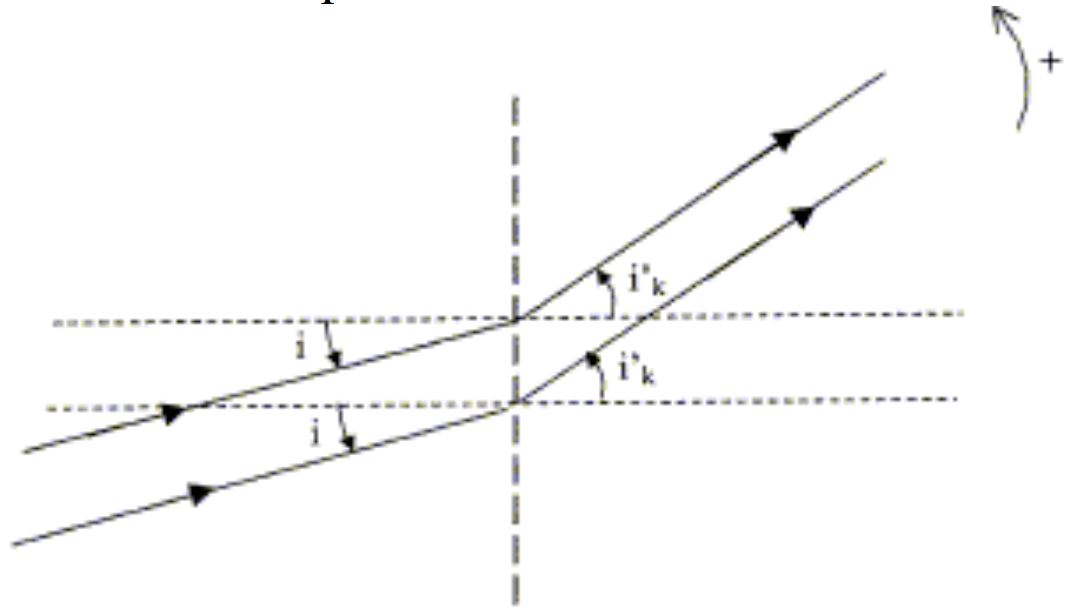
\includegraphics[width=\linewidth]{reseau}
  \end{center}
\end{tcb}
Ainsi, on ne voit de la lumière
que dans quelques directions, dont la direction incidente (pas de déviation,
$i=0$). L'examen de la formule des réseaux montre que $k$ est «~petit~»~: il ne
dépasse pas 2 ou 3 en général.

\begin{tcb}(impl){Implication}
  Si la lumière incidente est polychromatique, pour un ordre $k$ donné, l'angle
  $i_{k}'$ dépend de $\lambda$~: les différentes radiations sont donc
  angulairement séparées (sauf pour $k = 0$ où toutes les couleurs se
  superposent), et on obtient donc le spectre de la lumière incidente.
\end{tcb}

On note aussi que pour un ordre $k$ donné, à l'inverse du prisme, le violet est
moins dévié que le rouge. Ce constat n'est pas particulièrement surprenant
puisque ce n'est pas du tout les mêmes phénomènes physiques qui sont mis en jeu.
En effet, le prisme dévie la lumière de manière différenciée selon la fréquence
car l'indice optique du matériau qui le compose dépend de ladite fréquence. Dans
le cas du réseau, le phénomène est uniquement dû aux interférences entre un
grand nombre de sources.

\begin{tcb}(impo){}
  Dans le TP, \textbf{le réseau sera utilisé en incidence normale}, c'est-à-dire
  pour $i = 0$. Par ailleurs, le spectre sera établi autour du premier ordre
  d'interférence $k = \pm 1$.
\end{tcb}

\subsection{Présentation du goniomètre}

Un \textbf{goniomètre} est un appareil qui sert à \textbf{mesurer des angles}
avec une précision d'une minute d'angle. C'est donc un appareil adapté pour
évaluer les déviations de rayons lumineux par un réseau (ou un prisme).

\begin{tcb}(rapp){Rappel}
  \begin{center}
      $\ang{;60;} = \ang{1;;}$.
      Ainsi, on a donc~: $\ang{1.2;;}= \ang{1;12;}$ (par exemple).
  \end{center}
\end{tcb}

Un exemple de goniomètre est proposé ci-dessous. Il comporte~: 

\begin{itemize}
    \item Un \textbf{collimateur réglable}. Il créé un \textbf{objet à l'infini}
      à l'aide d'une fente éclairée avec une lampe spectrale et d'un objectif de
      distance focale $\SI{160}{mm}$.
      \smallbreak
      En tirant sur l'objectif, on peut placer la fente au foyer objet de ce
      dernier afin d'avoir une image à l'infini.
    \item Une \textbf{lunette autocollimatrice} montée sur un support mobile en
      rotation autour d'un axe central. Cette lunette de visée est constituée
      d'un objectif de distance focale $\SI{130}{mm}$ et d'un oculaire
      autocollimateur et permet de repérer un rayon émergent du réseau.
      L'horizontalité de l'axe de la lunette est réglable.
    \item Un plateau central, lui aussi mobile en rotation autour de l'axe
        central, monté sur un socle métallique fixe, le tout pouvant être rendu
        horizontal à l'aide de trois vis de réglage.
\end{itemize}

\begin{tcb}*(prop)"bomb"{}
  Puisqu'on cherche à effectuer des mesures précises, il est nécessaire de
  régler \textbf{parfaitement} l'appareil grâce à la démarche donnée ci-après.
  Cette démarche est longue et demande beaucoup de précisions. Soyez
  concentré-es car si vous faites mal une étape et que vous vous en rendez
  compte à l'étape 3, il faudra tout recommencer depuis le début…
\end{tcb}

\begin{center}
    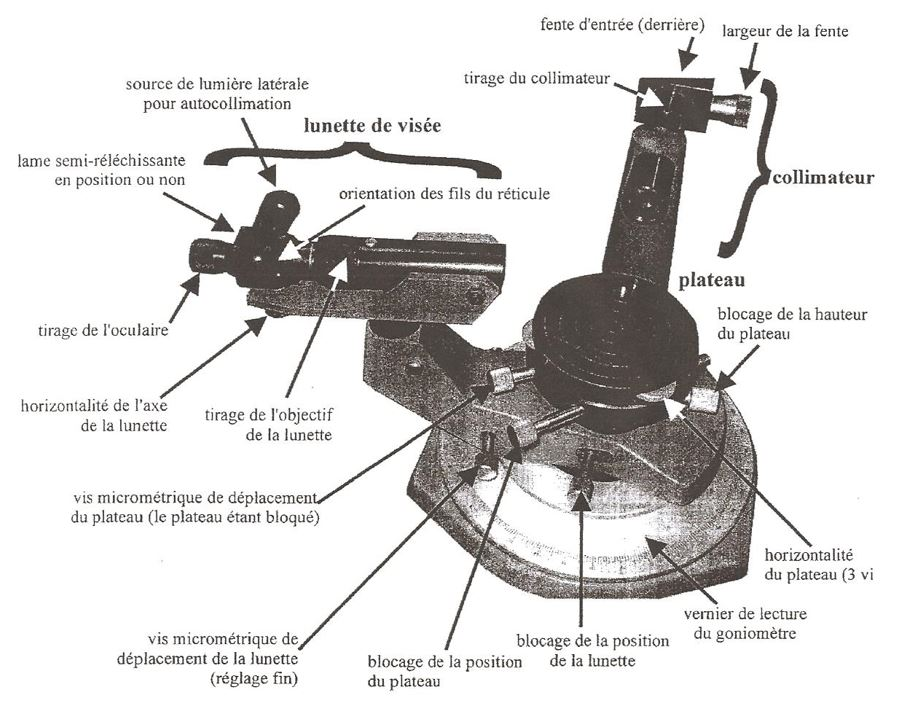
\includegraphics[width=0.8\textwidth]{goniometre}
\end{center}

\begin{tcb}(rema){}
  Les jurys d'épreuves de travaux pratiques aux concours adorent l'optique. Le
  matériel est facile à installer et l'évaluation est relativement simple~: le
  dispositif est bien réglé par læ candidat-e… ou pas~! Je vous invite donc à
  savoir faire ce réglage pour vos concours.
\end{tcb}

\section{Réaliser~: réglage du goniomètre}

\subsection{Horizontalité grossière du plateau}

Dans un premier temps, régler grossièrement (à l'œil) l'horizontalité du
plateau. En particulier, si l'une des vis de réglage semble particulièrement
vissée ou dévissée, la placer dans une position intermédiaire. 

\subsection{Réglage de la lunette autocollimatrice}

Cette lunette doit être réglée de façon à donner d'un \textbf{objet à l'infini}
une \textbf{image à l'infini} pour éviter toute fatigue de l'œil. Le système
doit donc être afocal.

\subsubsection{Régler l'oculaire à votre vue}

Allumer la lampe latérale de la lunette qui éclaire le réticule.
Régler l'oculaire à votre vue~: mettre au point le réticule en agissant sur
l'œilleton de l'oculaire. Ce réglage est personnel et nécessaire avant toute
manipulation~; La lunette est réglée quand on voit les deux fils croisés nets.


\subsubsection{Régler la lunette sur l'infini}

Positionner à la sortie de la lunette le petit miroir plan circulaire et tourner
la molette intermédiaire afin de régler la position de l'objectif  pour voir à
la fois le réticule et son image nets. Cette méthode est appelée
auto-collimation. 


\subsubsection{Régler l'horizontalité de la lunette (étape délicate~! )}

Le but de ce réglage est de rendre l'axe de la lunette orthogonal à l'axe de la
platine sans que celui-ci ne soit nécessairement vertical.

\begin{minipage}[c]{.45\linewidth}
  ~
  \begin{center}
    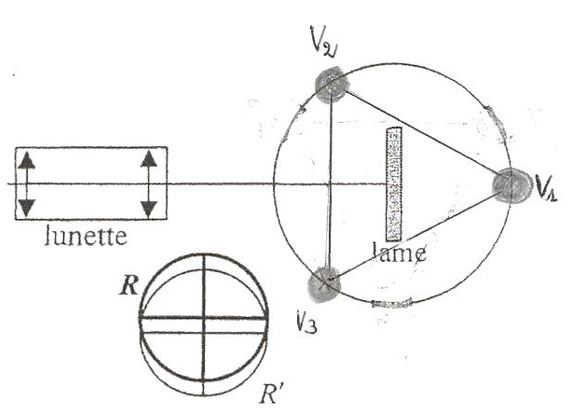
\includegraphics[width=\linewidth]{reglage1}
  \end{center}
\end{minipage}
\hfill
\begin{minipage}[c]{.45\linewidth}
  ~
  \begin{center}
    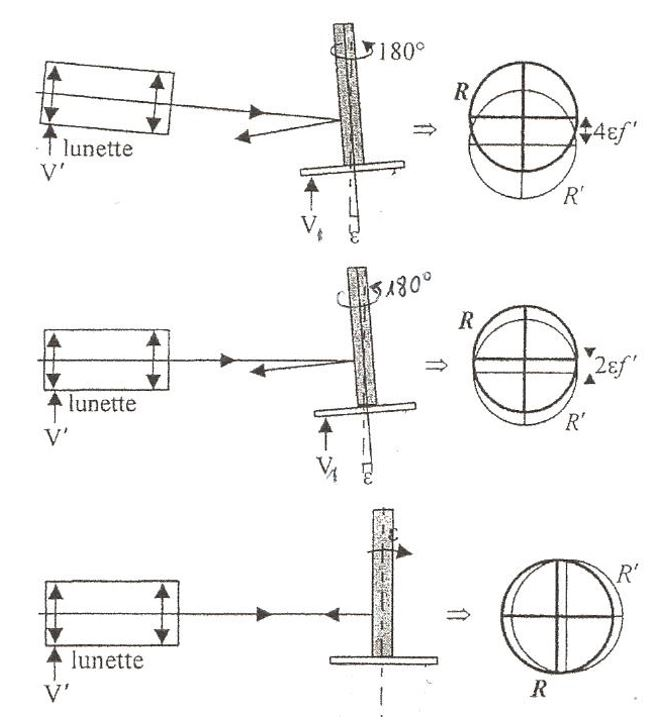
\includegraphics[width=\linewidth]{reglage2}
  \end{center}
\end{minipage}

\begin{tcb}(expe){}
  \begin{enumerate}
  \item Poser le miroir sans tain sur le plateau de façon à ce qu'elle soit
  approximativement parallèle à l'axe $V_2-V_3$. Viser à la lunette pour
  observer l'image du réticule. En général, le réticule $(R)$ et son image
  $(R')$ ne sont pas  confondus (cf.\ ci-dessus).

  \item En agissant sur la vis $V'$ de réglage de l'horizontalité de l'axe de
  la lunette (sous la lunette) et sur la vis $V_1$ du plateau, réduire l'écart
  initial entre $(R)$ et $(R')$ de sa \textbf{moitié}~: un quart en agissant sur
  $V'$ et un quart en agissant sur $V_1$. \textbf{Ne pas chercher à faire
  coïncider les deux réticules}.

  \item Tourner le plateau de $\ang{180;;}$. En général, l'image du fil
  horizontal $(R')$ ne coïncide pas encore avec $(R)$.

  \item Agir sur les deux mêmes vis de façon à diviser à nouveau l'écart entre
  les fils horizontaux par 2.

  \item Recommencer ainsi jusqu'à ce que les fils horizontaux de $(R)$ et
  $(R')$ coïncident de chaque côté. Le réglage de la lunette est alors terminé.
  Cinq à dix itérations sont souvent nécessaires. Notez que l'on cherche ici la
  coïncidence selon l'\textbf{horizontale}, pas selon la verticale.

  \end{enumerate}

\begin{tcb}*[bld, cnt](prop)"bomb"{}
  Ne plus toucher par la suite aux vis de réglages de la lunette~!
\end{tcb}

\begin{enumerate}[resume]
  \item Retirer ensuite le miroir sans tain du plateau. Basculer la lame
    semi-réfléchissante de la lunette autocollimatrice pour éteindre sa lampe.

  \item Allumer la lampe à vapeur de mercure (attention~: ne pas l'éteindre
    indûment, car, pour pouvoir la rallumer, il faudrait attendre qu'elle soit
    refroidie ce qui peut demander plusieurs minutes).
\end{enumerate}

\end{tcb}

\subsection{Réglage du tirage du collimateur}

Le collimateur doit donner de la fente une \textbf{image à l'infini}.
\begin{tcb}(expe){}
  \begin{enumerate}
    \item Diriger la lunette vers le collimateur $K$. Ouvrir la fente de
      $\SI{0,5}{mm}$ environ et l'éclairer par la source qui sera utilisée dans
      la manipulation suivante (ici, par la lampe à vapeur de mercure pour
      commencer).
    \item Observer alors l'image de la fente donnée par le collimateur à travers
      la lunette~:
    \begin{enumerate}
      \item Si le faisceau issu de $K$ est un faisceau de rayons parallèles,
    l'image donnée par $K$ est à l'infini (ce qui implique que la fente source
    soit dans le plan focal objet de $K$) et, dans la lunette, on observe une
    image nette de la fente dans le plan du réticule.
      \item Si ce n'est pas le cas, la fente est mal
    placée par rapport au collimateur, il faut déplacer la fente par tirage du
    collimateur jusqu'à ce que l'image dans la lunette soit nette (en
    particulier les bords de la fente).
    \end{enumerate}
    \begin{center}
      \bfseries
      Attention, vous ne devez plus toucher aux réglages de la lunette~! 
    \end{center}
    \item Refermer ensuite légèrement la fente, l'œil restant derrière l'oculaire
      de la lunette, de manière à observer un trait lumineux de faible largeur.
  \end{enumerate}
  \begin{tcb}*[bld, cnt](prop)"bomb"{}
    Ne plus toucher par la suite aux vis de réglages du tirage du collimateur~!
  \end{tcb}
  \begin{enumerate}[resume]
    \item Viser la position angulaire de la fente en superposant l'axe vertical
      de votre réticule sur la fente. Lire l'angle associé que l'on notera
      $\alpha_0$. C'est votre angle de référence pour toute la suite.
  \end{enumerate}
\end{tcb}

\subsection{Réglage de l'horizontalité du plateau (suite et fin)}

\begin{tcb}(expe){}
  \begin{enumerate}
    \item Poser le réseau au centre de la plate-forme,
      \textbf{perpendiculairement à la position du miroir sans tain que vous
      venez de retirer}. Basculer de nouveau la lame semi-réfléchissante et
      allumer la lampe de la lunette autocollimatrice.

    \item Observer l'image du réticule par réflexion sur le réseau (qui est de
      mauvaise qualité vu la nature de la surface du réseau). Faire tourner la
      plate-forme de façon à amener en coïncidence le fil vertical du réticule
      et son image. 

    \item Agir sur les vis $V_2$ et $V_3$ (attention il ne faut plus toucher à
      $V_1$ déjà réglée lors des précédentes étapes) d'inclinaison de la
      plate-forme pour amener le fil horizontal du réticule en coïncidence avec
      son image. Faire la rotation de $\ang{180;;}$ du plateau et recommencer
      l'opération. Quand les fils horizontaux de $(R)$ et $(R')$ coïncident de
      chaque côté, le plateau est horizontal.

    \item Basculer la lame semi-réfléchissante de la lunette, éteindre sa lampe,
      ouvrir légèrement la fente du collimateur, les mesures peuvent commencer.
  \end{enumerate}
\end{tcb}

\section{Réaliser~: Utiliser le goniomètre comme un spectromètre}

\subsection{Relevé des valeurs de déviation}

La première étape consiste à étalonner le goniomètre en déterminant la position
angulaire des raies spectrales de la lampe à vapeur de mercure. Tout d'abord,
nous allons positionner le réseau afin de se placer en indidence normale sur le
réseau. Pour ce faire, 

\begin{enumerate}
    \item Positionner la lunette d'observation précisément à l'angle $\alpha_0$. 

    \item Allumer de nouveau la lampe auxiliaire de la lunette, le réseau étant
        toujours positionné sur le plateau. La lunette étant toujours à la
        position $\alpha_0$, faire tourner le plateau afin que l'image du
        réticule se superpose parfaitement à lui-même dans la lunette. Eteindre
        la lampe auxiliaire. Le réseau est alors orthogonal au faisceau
        incident. Verrouiller le plateau, il ne devra absolument plus être
        touché.

    \item Observer le spectre d'ordre 1 ($k = 1$) en tournant la lunette.
        Relever les angles $\alpha$ correspondants aux raies visibles de
        différentes couleurs. Vous ouvrirez la fente afin de voir les raies les
        moins lumineuses puis la refermerez pour augmenter votre précision de
        pointé de chacune des raies.
\end{enumerate}

Le Tableau~\ref{tab:raiesint} suivant précise la longueur d'onde et l'intensité
(en unités arbitraires) des différentes raies visibles de la lampe à vapeur de
mercure. Il est possible que vous ne parveniez pas à toutes les observer.

\begin{table}[htbp]
  \centerfloat
  \caption{Intensité des raies.}
  \begin{tabular}{lccccccccc}
    \toprule
    Couleur &
    \multicolumn{2}{c}{Doublet violet} &
    Indigo &
    Vert-bleu &
    Vert &
    \multicolumn{2}{c}{Doublet jaune} &
    Rouge vermillon &
    Rouge carmin
    \\
    \midrule
    $\lambda$ (\si{nm}) &
    \num{404.7} &
    \num{407.8} &
    \num{435.8} &
    \num{491.6} &
    \num{546.1} &
    \num{577.0} &
    \num{579.1} &
    \num{623.4} &
    \num{690.7}
    \\
    Intensité &
    \num{1800} &
    \num{200} &
    \num{4400} &
    \num{100} &
    \num{1100} &
    \num{250} &
    \num{300} &
    \num{160} &
    \num{250}
    \\
    \bottomrule
  \end{tabular}
  \label{tab:raiesint}
\end{table}

\begin{enumerate}[label=\sqenumi]
  \item À partir de vos mesures, recopiez sur votre copie puis complétez le
    tableau suivant.
\end{enumerate}
\begin{table}[htbp]
  \centering
  \caption{Données à relever}
  \label{tab:raiesmes}
  \begin{threeparttable}
    \makebox[\linewidth]{%
    \begin{tabular}{lccccc}
      \toprule
      Couleur &
      $\lambda$ (\si{nm}) &
      $\alpha$ (\ang[parse-numbers=false]{x;y;}) &
      $\alpha$ (\ang[parse-numbers=false]{z;;}) &
      $i_1$\tnote{$\dag$} (\ang[parse-numbers=false]{x;;}) &
      $\sin(i_1)$
      \\
      \midrule
      Violet & $\ldots$ & $\ldots$ & $\ldots$ & $\ldots$ & $\ldots$
      \\
      $\ldots$ & $\ldots$ & $\ldots$ & $\ldots$ & $\ldots$ & $\ldots$
      \\
      $\ldots$ & $\ldots$ & $\ldots$ & $\ldots$ & $\ldots$ & $\ldots$
      \\
      $\ldots$ & $\ldots$ & $\ldots$ & $\ldots$ & $\ldots$ & $\ldots$
      \\
      $\vdots$ & $\vdots$ & $\vdots$ & $\vdots$ & $\vdots$ & $\vdots$
      \\
      \bottomrule
  \end{tabular}}
  \begin{tablenotes}[flushleft]
  \bitem{Notes.} $^\dag$On rappelle que $i_1 = \abs{\alpha-\alpha_0}$.
  \end{tablenotes}
  \end{threeparttable}
\end{table}

\subsection{Tracé de la courbe d'étalonnage}

\begin{enumerate}[label=\sqenumi, start=2]
  \item À l'aide de la méthode de votre choix (LatisPro, Regressi,
    Python\ftn{Activité \texttt{Capytale}~:
    \url{https://capytale2.ac-paris.fr/web/c/5d1d-1973717}}…), répresenter
    $\sin(i_1)$ en fonction de $\lambda$ puis montrer que la courbe est
    modélisable par une droite linéaire dont vous déterminerez le coefficient
    directeur et le coefficient de corrélation.
\end{enumerate}

\section{Valider~: Résolution du doublet jaune du sodium}
Changer de lampe et prendre dorénavant la lampe à vapeur de sodium.

\begin{enumerate}[label=\sqenumi, resume]
  \item Pour chacune des deux raies du doublet jaune du sodium, déterminer
    l'angle de déviation correspondant à l'ordre 1.

  \item En déduire alors les longueurs d'onde correspondantes à partir de la
    régression de la courbe d'étalonnage précédemment établie (vous donnerez vos
    résultats avec 4 chiffres significatifs). 

  Les valeurs tabulées pour le doublet du sodium sont $\lambda_1 =
  \SI{589,00}{nm}$ et $\lambda_2 = \SI{589,59}{nm}$.

  \item Calculer les écarts normalisés avec les valeurs trouvées
    expérimentalement. 

  \item Que pensez-vous de la précision de cet appareil~? Le prix d'achat est-il
    justifié~?
\end{enumerate}

\end{document}
